% !TEX root = ../main.tex
\chapter{GIỚI THIỆU CHUNG}
\label{chap:introduction}

\begingroup
\widowpenalty=10000

Chương này trình bày quá trình phát triển của quadrotor, nguyên lý tạo chuyển động và những vấn đề đặt ra khi thiết kế bộ điều khiển cân bằng. Trên cơ sở đó, đối tượng, phạm vi, phương pháp nghiên cứu và kết quả dự kiến của đề tài được xác định để làm cơ sở triển khai các chương tiếp theo.

\section{Lịch sử nghiên cứu và phát triển}
\label{sec:introduction-history}

Cấu hình thiết bị bay sử dụng bốn rôto đã xuất hiện từ đầu thế kỷ XX. Năm 1907, Gyroplane Breguet--Richet số 1 được thử nghiệm nâng khỏi mặt đất, song vẫn cần sự hỗ trợ từ người dưới mặt đất để duy trì ổn định~\cite{artsmetiers1907gyroplane}.

Sự phát triển của quadrotor cỡ nhỏ gắn liền với tiến bộ của cảm biến quán tính, cơ cấu chấp hành, nguồn điện và bộ xử lý nhúng. Vào đầu những năm 2000, việc tích hợp các thành phần này đã tạo điều kiện xây dựng những mô hình có khả năng thu nhận trạng thái chuyển động và ổn định tư thế bằng điều khiển phản hồi. Hướng nghiên cứu kết hợp thiết kế cơ khí, mô hình hóa động lực học, đo lường và điều khiển~\cite{bouabdallah2004design}.

Năm 2004, Bouabdallah, Murrieri và Siegwart công bố nghiên cứu về thiết kế và điều khiển quadrotor OS4 tại Trường Bách khoa Liên bang Lausanne (EPFL). Công trình trình bày kết cấu cơ khí, mô hình động lực học, hệ thống cảm biến và bệ thử phục vụ khảo sát bộ điều khiển. Mô hình OS4 trên bệ thử được minh họa trong \fref{fig:os4-test-bench}; việc giới hạn một số bậc tự do cho phép nghiên cứu chuyển động quay trước khi mở rộng sang thử nghiệm bay~\cite{bouabdallah2004design}.

\begin{figure}[htbp]
    \centering
    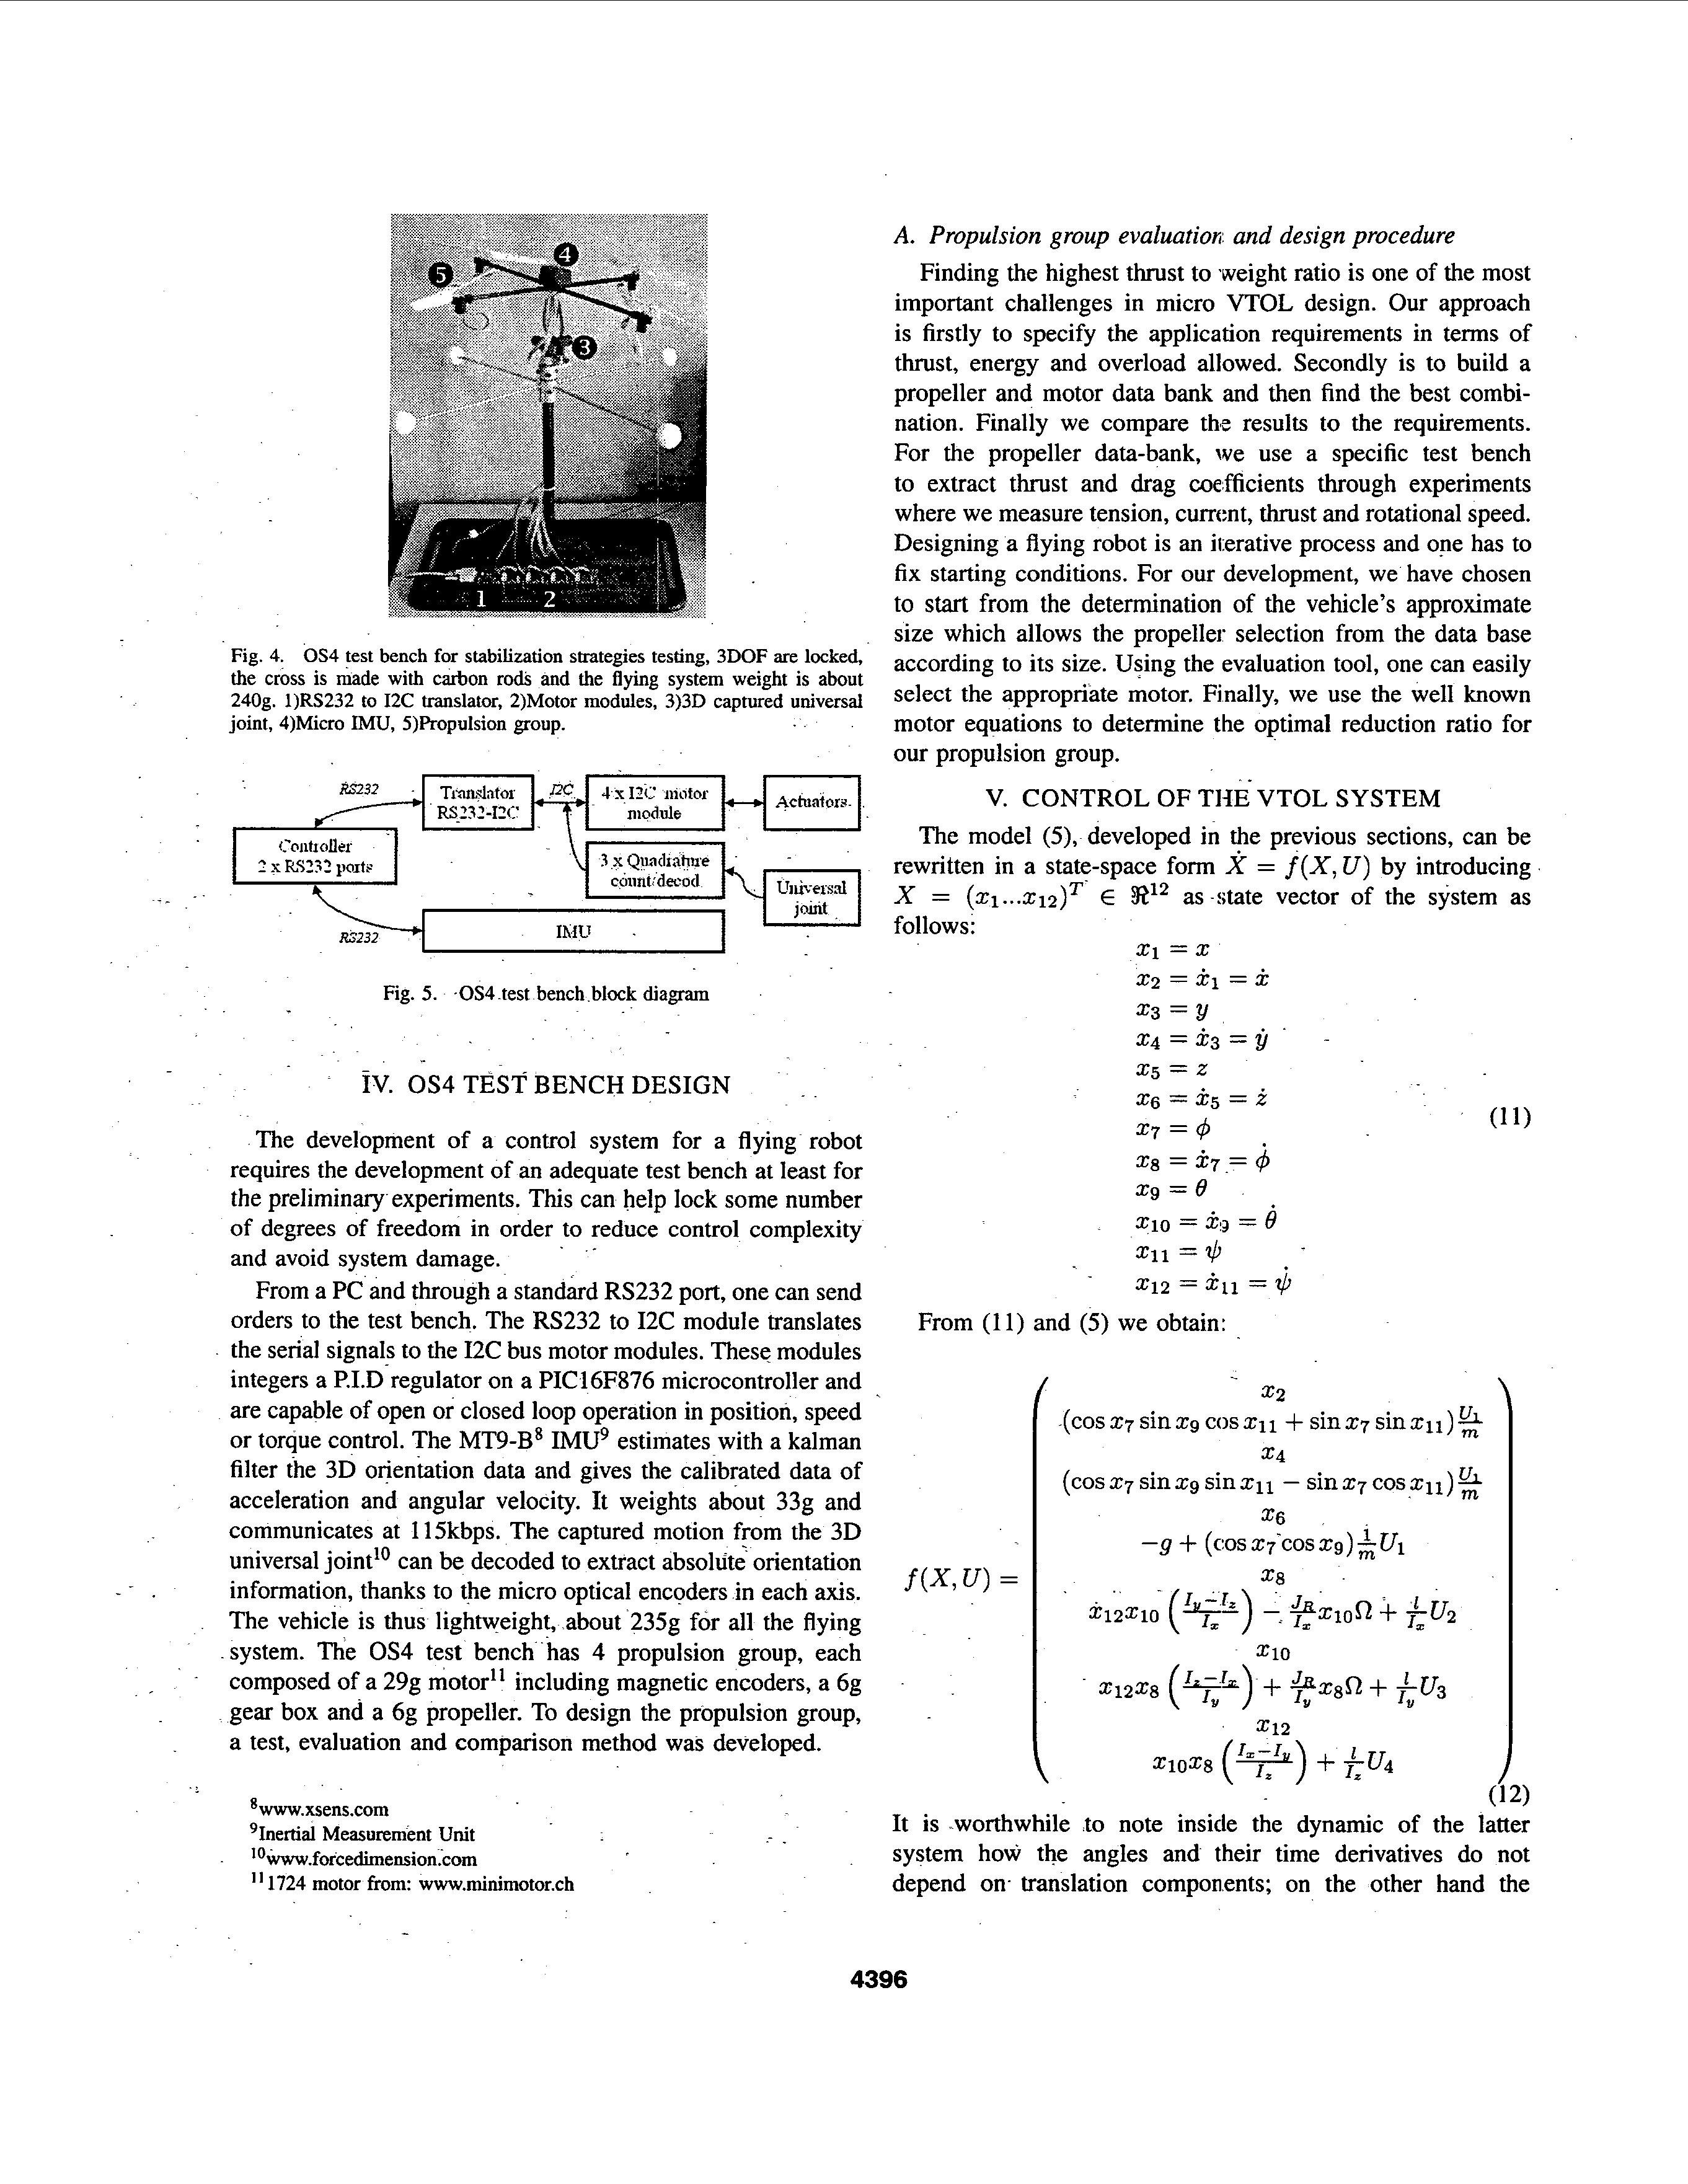
\includegraphics[width=0.40\linewidth,trim=625bp 2523bp 1578bp 340bp,clip]{figures/ch01/os4_test_bench_source-000.png}
    \caption[Mô hình quadrotor OS4 trên bệ thử nghiệm điều khiển tư thế.]{Mô hình quadrotor OS4 trên bệ thử nghiệm điều khiển tư thế~\cite{bouabdallah2004design}.}
    \label{fig:os4-test-bench}
\end{figure}

Cũng trong năm 2004, Bouabdallah, Noth và Siegwart khảo sát điều khiển tỉ lệ--tích phân--vi phân (PID) và điều khiển tối ưu tuyến tính toàn phương (LQ) cho OS4. Các phương án được xây dựng từ những mức độ giản lược mô hình khác nhau và được đánh giá bằng mô phỏng, thử nghiệm trên bệ cùng các kết quả thử bay ban đầu. Nghiên cứu cho thấy mô hình toán học và thực nghiệm có vai trò bổ sung cho nhau trong quá trình thiết kế bộ điều khiển~\cite{bouabdallah2004pidlqr}.

\clubpenalty=10000
Các nghiên cứu sau đó mở rộng từ ổn định tư thế sang điều khiển phi tuyến và bám quỹ đạo. Năm 2010, Lee, Leok và McClamroch đề xuất phương pháp điều khiển bám hình học trên nhóm Euclid đặc biệt $SE(3)$, biểu diễn đồng thời vị trí và tư thế của quadrotor. Việc sử dụng ma trận quay cho phép tránh điểm kỳ dị của biểu diễn góc Euler và xem xét chuyển động có góc quay lớn; các tính chất của hệ kín được phân tích lý thuyết và minh họa bằng mô phỏng~\cite{lee2010geometric}. Năm 2011, Mellinger và Kumar kết hợp sinh quỹ đạo theo tiêu chuẩn minimum snap với điều khiển phi tuyến để thực hiện bám quỹ đạo ba chiều, đồng thời kiểm chứng bằng thực nghiệm~\cite{mellinger2011minimum}.

Ở Việt Nam, bài toán mô hình hóa và điều khiển quadrotor cũng được nghiên cứu theo nhiều hướng. Năm 2024, Hoàng Văn Huy trình bày mô hình động lực học có xét cơ cấu chấp hành là động cơ điện một chiều với bộ điều khiển thích nghi, đồng thời mô phỏng hệ điều khiển trên MATLAB/Simulink. Công trình là một ví dụ về việc xét thêm đặc tính cơ cấu chấp hành khi xây dựng hệ điều khiển quadrotor~\cite{huy2024simulation}.

Những công trình trên thể hiện sự phát triển từ thiết kế mô hình và ổn định tư thế đến các bài toán điều khiển có yêu cầu cơ động cao. Đối với đề tài này, mô hình hóa động lực học và điều khiển tư thế là cơ sở tham khảo trực tiếp. Hướng tiếp cận được lựa chọn là tập trung vào góc roll và pitch trong miền góc nghiêng nhỏ, tạo nền tảng để triển khai bộ điều khiển trên vi điều khiển và đánh giá bằng dữ liệu của hệ thống.

\section{Nguyên lý hoạt động}
\label{sec:introduction-principle}

Quadrotor sử dụng bốn cụm động cơ--cánh quạt bố trí quanh thân để tạo lực đẩy và mômen điều khiển. Trong cấu hình thông dụng, các trục rôto song song với nhau; hai rôto đối diện quay cùng chiều, còn hai rôto kề nhau quay ngược chiều. Khi mômen phản lực của hai nhóm quay ngược chiều cân bằng, tổng mômen quanh trục đứng của thân máy bay được triệt tiêu trong điều kiện lý tưởng. Chuyển động được điều khiển bằng cách thay đổi tốc độ quay của từng rôto~\cite{bouabdallah2004design}.

\fref{fig:quadrotor-principle} minh họa một cấu hình chữ X nhìn từ trên xuống. Hệ trục gắn với thân máy bay gồm trục dọc $x_B$ hướng về phía mũi, trục ngang $y_B$ hướng sang phải và trục $z_B$ hướng xuống dưới. Trong lân cận tư thế nằm ngang, chuyển động roll, pitch và yaw lần lượt tương ứng với chuyển động quay quanh các trục này. Số thứ tự rôto và chiều quay trên hình được dùng làm quy ước minh họa nguyên lý.

\begin{figure}[htbp]
    \centering
    \begin{tikzpicture}[
    x=1cm,y=1cm,
    >=latex,
    line width=0.8pt,
    font=\fontsize{11}{13}\selectfont,
    every node/.style={align=center}
]
    % Schematic convention for this figure; viewed from above.
    \draw[gray!55,line width=8pt,line cap=round] (-2,-2) -- (2,2);
    \draw[gray!55,line width=8pt,line cap=round] (-2,2) -- (2,-2);
    \draw[fill=gray!10,rounded corners=2pt] (-0.48,-0.48) rectangle (0.48,0.48);

    % Opposite rotors rotate in the same direction.
    \foreach \x/\y/\n in {-2/2/1,2/-2/3}{
        \begin{scope}[shift={(\x,\y)}]
            \draw[fill=white] (0,0) circle (0.73);
            \draw[->,line width=1pt] (130:0.87) arc (130:-130:0.87);
            \node at (0,0.19) {Rôto \n};
            \node at (0,-0.22) {CW};
        \end{scope}
    }
    \foreach \x/\y/\n in {2/2/2,-2/-2/4}{
        \begin{scope}[shift={(\x,\y)}]
            \draw[fill=white] (0,0) circle (0.73);
            \draw[->,line width=1pt] (50:0.87) arc (50:310:0.87);
            \node at (0,0.19) {Rôto \n};
            \node at (0,-0.22) {CCW};
        \end{scope}
    }

    % Body frame: x points forward, y points right, z points into the page.
    \draw[->] (0,0) -- (0,3.15) node[above] {$x_B$ -- hướng mũi};
    \draw[->] (0,0) -- (3.6,0) node[right] {$y_B$};
    \draw[fill=white] (0,0) circle (0.13);
    \draw (-0.085,-0.085) -- (0.085,0.085);
    \draw (-0.085,0.085) -- (0.085,-0.085);
    \node[anchor=north west] at (0.52,-0.32) {$z_B$};

    \node[anchor=west,align=left] at (3.15,2.0)
        {Roll: quay quanh $x_B$\\Pitch: quay quanh $y_B$\\Yaw: quay quanh $z_B$};
    \node[anchor=west,align=left] at (3.15,-1.7)
        {$\otimes\;z_B$: hướng vào trang\\CW: cùng chiều kim đồng hồ\\CCW: ngược chiều kim đồng hồ};
\end{tikzpicture}

    \caption{Sơ đồ bố trí rôto và các trục của quadrotor cấu hình chữ X, nhìn từ trên xuống.}
    \label{fig:quadrotor-principle}
\end{figure}

Khi thay đổi đồng thời lực đẩy của cả bốn rôto, tổng lực tác dụng theo phương trục rôto thay đổi. Ở tư thế nằm ngang, tổng lực đẩy cân bằng trọng lực là điều kiện cân bằng lực theo phương thẳng đứng; khi lực đẩy lớn hơn hoặc nhỏ hơn trọng lực, máy bay có gia tốc tương ứng theo phương này. Để tạo mômen roll, bộ điều khiển điều chỉnh chênh lệch lực đẩy giữa các rôto ở hai phía trái và phải. Tương tự, chênh lệch lực đẩy giữa phía trước và phía sau tạo mômen pitch. Với cấu hình chữ X, mỗi rôto đều tham gia tạo mômen quanh cả trục dọc và trục ngang, nên lệnh điều khiển được phân bổ đồng thời cho bốn động cơ.

Chuyển động yaw được tạo ra bằng chênh lệch tổng mômen phản lực giữa hai nhóm rôto quay ngược chiều. Khi thân máy bay nghiêng, vectơ tổng lực đẩy cũng nghiêng theo và xuất hiện thành phần lực theo phương ngang. Vì vậy, điều khiển tư thế có ảnh hưởng trực tiếp đến chuyển động tịnh tiến. Đây là đặc điểm quan trọng của quadrotor: hệ thống có sáu bậc tự do nhưng chỉ có bốn đầu vào điều khiển độc lập, gồm tổng lực đẩy và ba thành phần mômen~\cite{bouabdallah2004design}.

Để duy trì tư thế mong muốn, hệ thống sử dụng thông tin phản hồi từ cảm biến. Dữ liệu gia tốc và vận tốc góc được xử lý để ước lượng góc roll, pitch; sai lệch giữa góc đặt và góc ước lượng được đưa vào bộ điều khiển. Kết quả tính toán được phân bổ thành lệnh cho các động cơ, qua đó tạo mômen hiệu chỉnh. \fref{fig:attitude-control-loop} thể hiện mối liên hệ giữa các khối chức năng ở mức tổng quát; mô hình toán học và cấu trúc các vòng điều khiển được trình bày trong \charef{chap:background} và \charef{chap:system-design}.

\begin{figure}[htbp]
    \centering
    \begin{tikzpicture}[
    x=1cm,y=1cm,
    >=latex,
    line width=0.8pt,
    font=\fontsize{11}{13}\selectfont,
    block/.style={draw,fill=gray!6,minimum height=1.15cm,
        text width=2.6cm,inner sep=4pt,align=center},
    every node/.style={align=center}
]
    \node[draw,circle,minimum size=0.48cm,inner sep=0pt] (sum) at (1.3,0) {};
    \node[block] (controller) at (3.65,0) {Bộ điều khiển\\ổn định tư thế};
    \node[block] (allocation) at (7.1,0) {Phân bổ lệnh\\cho động cơ};
    \node[block] (plant) at (10.55,0) {Động cơ và\\thân quadrotor};
    \node[block,text width=3.5cm] (estimation) at (8.0,-2.05)
        {Cảm biến và\\ước lượng tư thế};

    \draw[->] (-0.2,0) -- (sum.west);
    \node at (0.25,0.62) {Góc đặt\\$\phi_d,\theta_d$};
    \node at (0.91,0.28) {$+$};
    \node at (1.0,-0.38) {$-$};
    \draw[->] (sum.east) -- (controller.west);
    \node at (1.9,0.3) {$e$};
    \draw[->] (controller.east) -- (allocation.west);
    \draw[->] (allocation.east) -- (plant.west);
    \draw[->] (plant.east) -- (13.1,0);
    \node at (13.0,0.62) {Tư thế\\$\phi,\theta$};

    \draw[->] (12.4,0) |- (estimation.east);
    \fill (12.4,0) circle (1.5pt);
    \draw[->] (estimation.west) -| (sum.south);
    \node at (3.7,-1.68) {Góc ước lượng $\hat\phi,\hat\theta$};
\end{tikzpicture}

    \caption{Sơ đồ nguyên lý điều khiển phản hồi góc roll và pitch.}
    \label{fig:attitude-control-loop}
\end{figure}

\section{Các vấn đề đặt ra và mục tiêu nghiên cứu}
\label{sec:introduction-objectives}

Vấn đề đầu tiên là xác định mô hình phù hợp để mô tả quan hệ giữa lực đẩy, mômen và chuyển động quay của quadrotor. Mô hình phải phản ánh được các yếu tố chi phối đáp ứng tư thế, đồng thời có mức độ phức tạp phù hợp với việc thiết kế và triển khai bộ điều khiển. Khối lượng, vị trí trọng tâm, mômen quán tính và đặc tính của cụm động cơ--cánh quạt là những yếu tố ảnh hưởng đến quan hệ này. Sai lệch giữa mô hình và hệ thống thực có thể làm thay đổi đáp ứng sau khi lựa chọn các hệ số điều khiển.

Vấn đề tiếp theo là thu nhận thông tin phản hồi đủ tin cậy. Con quay hồi chuyển cung cấp vận tốc góc nhưng sai lệch đo có thể tích lũy khi tích phân để tính góc; gia tốc kế cung cấp thông tin liên quan đến phương trọng lực nhưng chịu ảnh hưởng của rung động và gia tốc chuyển động. Việc kết hợp và lọc dữ liệu phải cân bằng giữa khả năng giảm nhiễu với độ trễ của tín hiệu. Bên cạnh đó, giới hạn lệnh động cơ và thời gian thực hiện chương trình trên vi điều khiển ảnh hưởng đến khả năng đáp ứng của vòng điều khiển.

Từ các vấn đề trên, mục tiêu tổng quát của đề tài là xây dựng cơ sở mô hình hóa và thiết kế bộ điều khiển ổn định tư thế cho quadrotor, tập trung vào điều khiển góc roll và pitch trong lân cận tư thế nằm ngang. Bộ điều khiển hướng đến duy trì các góc tại giá trị đặt và hiệu chỉnh sai lệch để khôi phục tư thế mong muốn khi có tác động làm lệch góc.

Để thực hiện mục tiêu đó, đề tài xác lập hệ tọa độ và mô hình động lực học phục vụ thiết kế; xây dựng phương án thu nhận, hiệu chỉnh và xử lý dữ liệu cảm biến; lựa chọn cấu trúc điều khiển và phương pháp phân bổ lệnh cho bốn động cơ. Cấu trúc điều khiển xếp tầng, gồm vòng góc bên ngoài và vòng vận tốc góc bên trong, được lựa chọn để nghiên cứu, trong đó PID là phương án tập trung khảo sát cho vòng trong. Khả năng đáp ứng được đánh giá qua sai lệch góc, mức dao động, độ quá điều chỉnh, thời gian xác lập và khả năng khôi phục tư thế sau tác động nhiễu.

\section{Đối tượng và phạm vi nghiên cứu}
\label{sec:introduction-scope}

Đối tượng nghiên cứu là hệ thống điều khiển tư thế của quadrotor, bao gồm động lực học quay của thân máy bay, các cụm động cơ--cánh quạt, cảm biến quán tính và bộ điều khiển thực hiện trên vi điều khiển STM32. Mối quan hệ giữa phần cơ khí, tín hiệu đo và thuật toán điều khiển được xem xét nhằm xây dựng một hệ thống có thể triển khai và đánh giá trên mô hình của đề tài.

Phạm vi mô hình hóa tập trung vào chuyển động quay quanh các trục thân máy bay. Thân máy bay được xem là vật rắn; điều kiện làm việc được giới hạn trong miền góc roll và pitch nhỏ quanh tư thế nằm ngang. Trên cơ sở này, mô hình được giản lược để phục vụ thiết kế bộ điều khiển và phân tích đáp ứng. Các kết luận về chất lượng điều khiển được gắn với miền làm việc và điều kiện thử nghiệm tương ứng, không mở rộng sang chuyển động cơ động có góc nghiêng lớn.

Phạm vi thực hiện gồm xử lý dữ liệu quán tính, ước lượng roll và pitch, tính toán tác động điều khiển, phân bổ lệnh động cơ và ghi nhận các đại lượng phục vụ đánh giá. Điều khiển góc hướng yaw được xem xét như nội dung bổ sung theo cấu hình cảm biến và yêu cầu thiết kế. Giữ độ cao, giữ vị trí, dẫn đường và bay tự động được xác định là những hướng phát triển tiếp theo; việc đánh giá trong đề tài tập trung vào khả năng ổn định tư thế.

\section{Phương pháp nghiên cứu}
\label{sec:introduction-methods}

Đề tài kết hợp nghiên cứu tài liệu, phân tích và mô hình hóa toán học, triển khai thuật toán trên vi điều khiển và thực nghiệm trên mô hình vật lý. Việc khảo sát tài liệu tập trung vào nguyên lý quadrotor, động lực học vật rắn, ước lượng tư thế và điều khiển phản hồi. Các công trình đã công bố được sử dụng để lựa chọn cách biểu diễn trạng thái, cấu trúc bộ điều khiển và phương thức kiểm chứng phù hợp với mục tiêu roll, pitch góc nhỏ.

Phương pháp mô hình hóa dựa trên các quan hệ lực và mômen tác dụng lên thân máy bay. Sau khi thống nhất hệ tọa độ, chiều dương và ký hiệu, các phương trình chuyển động được thiết lập và giản lược quanh điều kiện làm việc đã chọn. Mô hình này là cơ sở phân tích ảnh hưởng của tham số và lựa chọn ban đầu các hệ số điều khiển. Đối với dữ liệu cảm biến, phương án xử lý được xây dựng từ việc hiệu chỉnh sai lệch đo và kết hợp thông tin gia tốc với vận tốc góc để ước lượng tư thế.

Thuật toán được triển khai trên STM32 theo các chức năng thu nhận dữ liệu cảm biến, ước lượng tư thế, tính toán điều khiển và phân bổ lệnh động cơ. Quá trình kiểm tra được thực hiện từ từng khối chức năng đến vòng điều khiển hoàn chỉnh. Dữ liệu cảm biến, chiều tác động của lệnh động cơ và chu kỳ thực hiện chương trình được kiểm tra trước khi khảo sát khả năng ổn định tư thế trên mô hình có giới hạn chuyển động phù hợp.

Thực nghiệm điều khiển tập trung khảo sát đáp ứng khi thay đổi góc đặt, khi có sai lệch tư thế ban đầu và khi có tác động làm lệch góc. Góc đặt, góc ước lượng, vận tốc góc và lệnh động cơ được ghi nhận theo thời gian. Các hệ số điều khiển được hiệu chỉnh dựa trên đáp ứng đo được, đồng thời xét giới hạn tác động điều khiển. Dữ liệu thực nghiệm là cơ sở đánh giá sai lệch góc, mức dao động, độ quá điều chỉnh, thời gian xác lập và khả năng khôi phục tư thế; điều kiện thử và cách xác định các chỉ tiêu được trình bày tại \charef{chap:evaluation}.

\section{Dự kiến kết quả đạt được}
\label{sec:introduction-expected-results}

Về lý thuyết, đề tài dự kiến xây dựng được mô hình động lực học phục vụ điều khiển tư thế quadrotor, thống nhất các quy ước về hệ tọa độ, góc quay và đầu vào điều khiển. Mô hình làm rõ quan hệ giữa lệnh tác động lên các động cơ với mômen quay và đáp ứng roll, pitch trong miền góc nghiêng nhỏ.

Về thiết kế, kết quả dự kiến là phương án điều khiển gồm các khối thu nhận dữ liệu quán tính, ước lượng tư thế, điều khiển xếp tầng và phân bổ lệnh động cơ. Chương trình trên STM32 dự kiến thực hiện các chức năng này theo chu kỳ xác định, đồng thời cung cấp dữ liệu để theo dõi và hiệu chỉnh hệ thống.

Về đánh giá, đề tài hướng đến thu được dữ liệu đo đạc và các đồ thị đáp ứng thực nghiệm thể hiện khả năng duy trì góc đặt, hiệu chỉnh sai lệch roll, pitch và khôi phục tư thế sau tác động nhiễu trong điều kiện khảo sát. Các chỉ tiêu được xác định từ dữ liệu thực nghiệm để đánh giá mức độ đạt mục tiêu, giới hạn của phương án và cơ sở phát triển hệ thống trong các nghiên cứu tiếp theo.
\par
\endgroup
